\section{Object Selection Criteria}
\label{sec:criteria}
In producing our candidate sample, we must consider our likely physical sources of contamination, and how removing those sources reduces the completeness of our criteria. Using the sample sets from Section~\ref{sec:merged}, we consider sample completeness and contamination in Section~\ref{sec:comp_cont} and devise simple criteria in WISE-2MASS color-color space. YSOs and RGBs present a special case of IR contaminants, as they are fairly well embedded in the same color-color regions as AGB stars. We consider the special case of YSOs in Section~\ref{sec:kill_ysos}, developing finer criteria to remove these objects while still preserving as much of the AGB sample as possible. We do the same with RGBs in Section~\ref{sec:kill_rgbs}.

\subsection{Completeness and Contamination of Initial Samples}\label{sec:comp_cont}
Sample completeness $\eta$ is defined as
\begin{eqnarray*}
\eta &=& \frac{N - n_\text{missed}}{N}
\end{eqnarray*}
where $N$ is the total number of objects in the sample, and $n_\text{missed}$ is the number of objects outside of the applied boundaries. \cite{2013sdmm.book.....I} defines sample contamination as
\begin{eqnarray*}
\epsilon &=& \frac{n_\text{spurious}}{n_\text{selected}}.
\end{eqnarray*}
where $n_\text{spurious}$ is the number of spurious sources and $n_\text{selected} = N + n_\text{spurious}$. Our primary goal is to get an acceptably low contamination of the AGB sample ($\le$2\% contamination) while still retaining a large number of AGB stars.

The difficulty with determining contamination is that none of the contaminant sample, save for the locus stars,  falls within the region occupied by our AGB sample: the LMC. However, knowing that there is essentially a uniform distribution of extragalactic sources on the sky {\color{red}[a citation would be great]}, we solve for the number density of objects in the 10,417 sq. deg. DR7 footprint. We then scale these number densities up by the $\sim76.5$ deg$^2$ area occupied by the LMC. This should provide a reasonable estimate for the number of sources that we would find within the region of the LMC, and by consequence estimate our final levels of extragalactic contamination in WISE-2MASS color-color space. 

We employ the following color criteria to isolate AGB stars from their potential contaminants:
\begin{eqnarray}
&(J - K_s) &>\;\;1.1\label{eq:criteria1}\\
0.2\;<&(W2 - W3) &<\;\; 2.5\label{eq:criteria2}
\end{eqnarray}
\noindent Figure~\ref{fig:colorcuts} shows completeness distributions for the OGLE-2MASS-WISE AGB sample, and corresponding contamination distributions for the contaminant samples. YSOs are omitted as they were not objects that could be projected to the LMC. Table~\ref{tab:criteria_completeness_contamination} shows the completeness and contamination fractions for each color criterion. We include the lower limit in ($W2-W3$) because, although there's a higher penalty on completeness and a slight increase in contamination, we want to exclude the spike of locus stars with ($W2-W3$) $< 0.2$.

\begin{figure}[h]
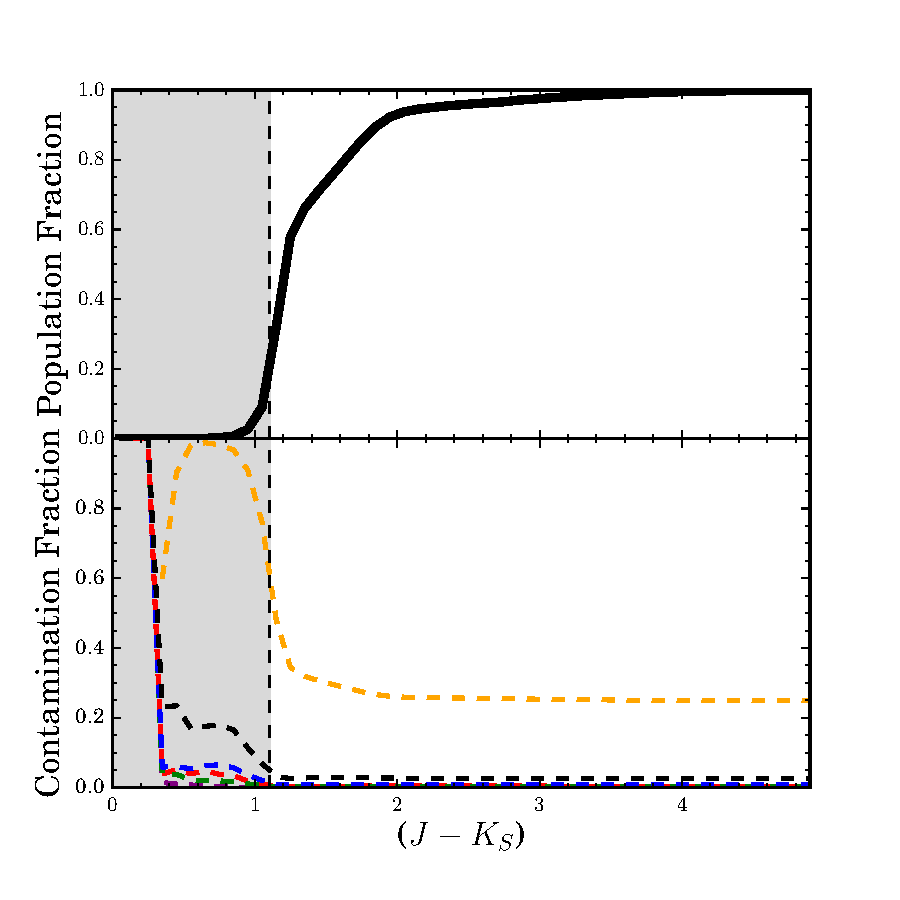
\includegraphics[width=3.3in]{figs/completeness_contamination_jkcut.pdf}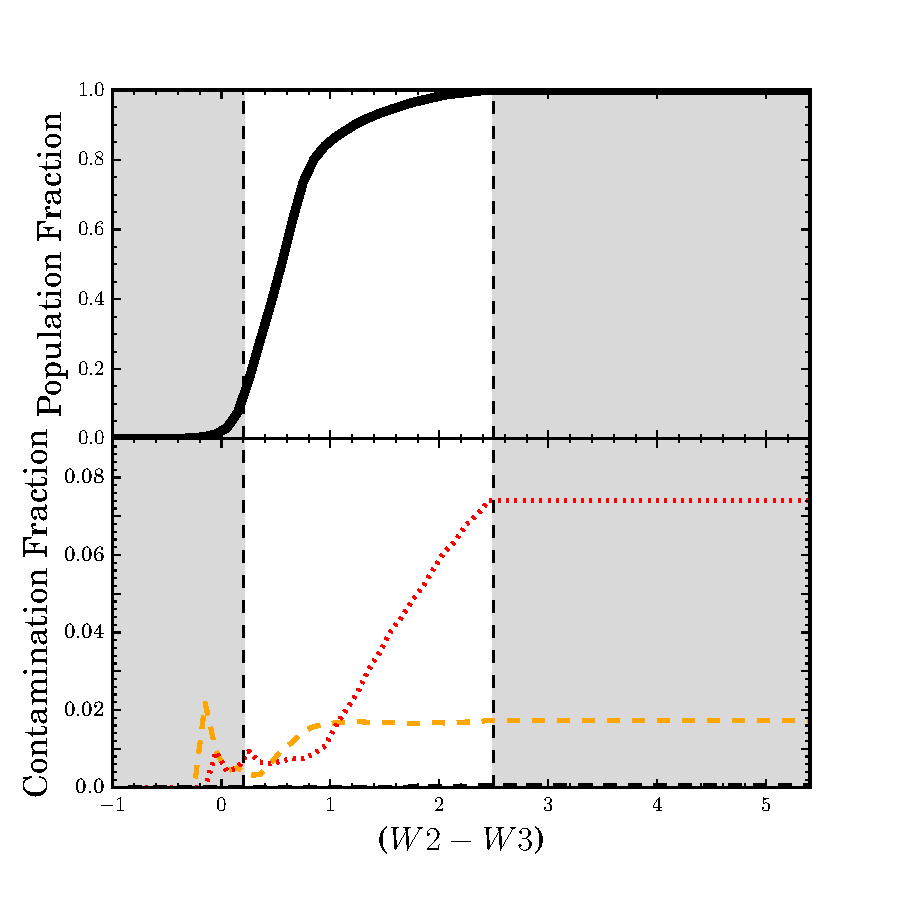
\includegraphics[width=3.3in]{figs/completeness_contamination_allcuts.pdf}
\caption{\emph{Left:} Cumulative completeness and contamination distributions before $(J-K_s)$ color cut. \emph{Right:} Cumulative completeness and contamination after $(J-K_s)$ and $(W2-W3)$ cuts. Thick black line in top panels is OGLE-2MASS-WISE AGB completeness as a function of color. The bottom panels show the contamination distributions with respect to color for stellar locus stars (\emph{orange, dashed}), RGB stars (\emph{red, dotted}), LRGs (\emph{purple, dashed}), QSOs (\emph{red, dashed}), AGN (\emph{green, dashed}), starforming galaxies (\emph{black, dashed}), and starburst galaxies (\emph{blue, dashed}). Bin width for both panels is 0.1 dex.  Shaded regions represent the color-color space affected by equations~\ref{eq:criteria1} \& \ref{eq:criteria2}. \label{fig:colorcuts}}
\end{figure}

\begin{table}[h]
	\begin{center}
	\scalebox{0.85}{		
		\begin{tabular}{l r r r r r r r r}
		\hline\hline
		Critiera & QSO & AGN & LRG & SF & SB & Locus & RGB & \textbf{AGB Completeness}\\
		\hline
		$(J-K_s) > 1.1$ & 0.25\% & 0.13 \%& 0.08\% & 0.56\% & 0.33\% & 4.86\% & 9.65\% &91.29\%\\
		$(W2-W3) < 2.5$ & 0.03\% & $<0.01$\%& 0.04\% & 0.05\% & 0.01\% & 1.73\% & 7.41\% &90.03\% \\
		$(W2-W3) > 0.2$ & 0.03\% & $<0.01$\%& 0.05\% & 0.06\% & 0.02\% & 1.83\% & 7.94\% &83.13\% \\

		\hline\hline
		\end{tabular}
		}    
	\caption{Sample contamination and completeness (\emph{bold}) with respect to each successive cut on WISE-2MASS color.\label{tab:criteria_completeness_contamination}}
	\end{center}
\end{table}

Figure~\ref{fig:lmc_completeness} shows the distribution of recovered AGB stars on the sky as well as in color-color space. We reserve a full accounting of YSOs and RGBs for the next subsections, as there is significant overlap between YSOs, RGBs, and AGBs, and they are not evenly distributed across the sky.

\begin{figure}[h]
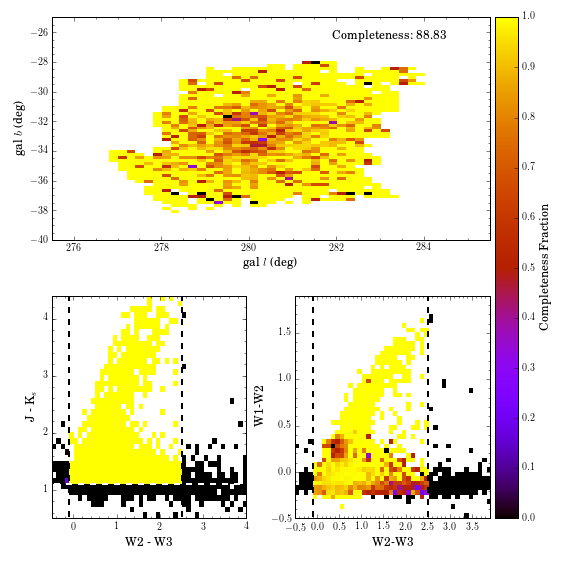
\includegraphics[width=6in]{figs/ogle_completeness_map.png}
\caption{Completeness fraction distributions for AGB stars in the LMC. \emph{Top:} OGLE-III AGB completeness fractions with position. Bin size is 0.2 deg on each axis. \emph{Bottom:} completeness  fractions in color-color space. Dashed lines represent the primary AGB candidate criteria in equations~\ref{eq:criteria1} \& \ref{eq:criteria2}. Bin size is 0.1 dex on each axis. \label{fig:lmc_completeness}}
\end{figure}

\subsection{Accounting for YSOs}\label{sec:kill_ysos}
YSOs often directly overlap with AGB stars in WISE color-color space, so we treat these objects separately from our  extragalactic contaminants. \cite{2011ApJS..196....4R} produced a catalog of YSOs in the Taurus Molecular Cloud to bring the total number of YSOs in that region up to 290. We use these and the AGB candidate criteria from Section~\ref{sec:comp_cont} to further refine our criteria and increase the purity of our sample.

\begin{figure}[h]
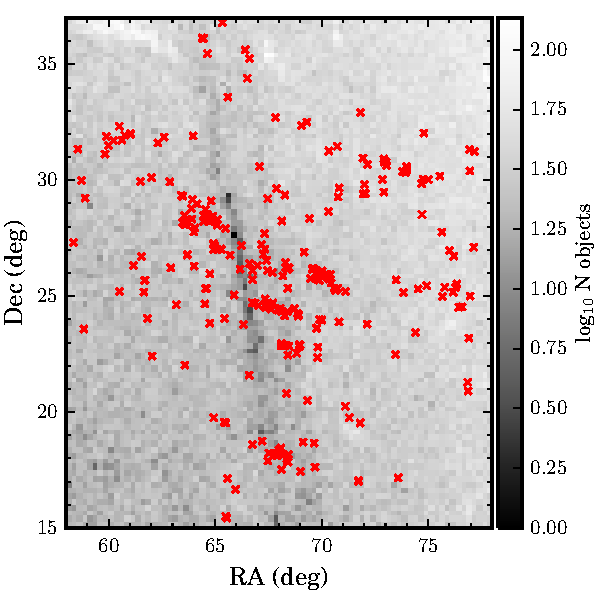
\includegraphics[width=4in]{figs/taurus_field_YSOs.pdf}
\caption{YSOs (\emph{red x}) in the Taurus Molecular Cloud (\emph{background}), sampled from \citep{2011ApJS..196....4R}.\label{fig:yso_field}}
\end{figure}
\begin{figure}[h]
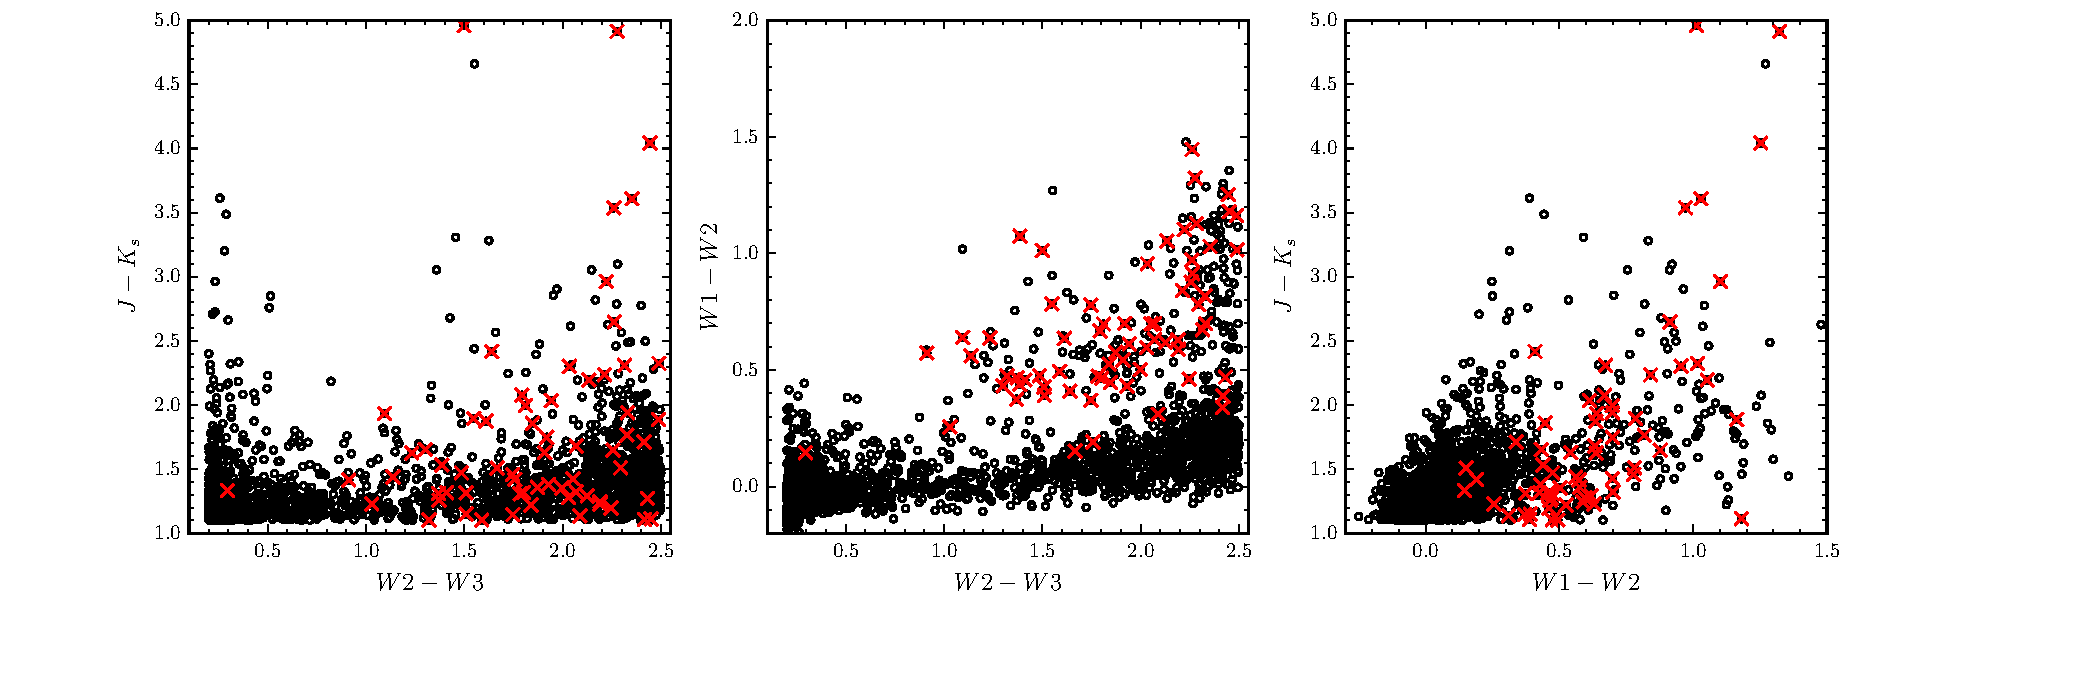
\includegraphics[width=6.5in]{figs/ysos_taurus_color.pdf}
\caption{YSOs (\emph{red x}) and AGB candidates (\emph{black o}) in the Taurus Molecular Cloud. \label{fig:ysos_agbs_taurus}}
\end{figure}

Figure~\ref{fig:yso_field} shows these 290 YSOs in the field of the Taurus Molecular Cloud, overplotted on WISE objects in that field. As shown in Table~\ref{tab:reductions}, after photometric and quality cuts we are left with 174 YSOs, and only 68 after applying equations~\ref{eq:criteria1} \& \ref{eq:criteria2}. In contrast, applying equations~\ref{eq:criteria1} \& \ref{eq:criteria2} as well as photometric criteria from Section~\ref{sec:merged} to the WISE field in the Taurus Molecular Cloud yields 2,195 AGB candidates in that field. Figure~\ref{fig:ysos_agbs_taurus} shows the degree of entanglement in color-color space for YSOs and AGB candidates. However, we note that because these are galactic AGB candidates, and the Milky Way is deficient in C-rich AGB stars [XXX CITATION HERE XXX], Figure~\ref{fig:ysos_agbs_taurus} misses the degree to which YSOs contaminate the C-rich sequence of AGB stars. To clarify, we compare Taurus YSOs to AGB stars from the LMC (Figure~\ref{fig:ysos_lmc}). Based on their positions in color-color space, we add three more constraints to remove YSOs from our AGB candidate sample:

\begin{align}
(W1-W2) &< 0.75(W2-W3) - 0.33 & \text{for } (W2-W3) > 1.075\label{eq:yso_criteria1}\\
(W1-W2) &> -(W2-W3) + 1.5 & \text{for }(W2-W3) > 1.075\label{eq:yso_criteria2}\\
(W1-W2) &> 0.2 & \text{for }(W2-W3) > 1.3\label{eq:yso_criteria3}
\end{align}

Collectively, these criteria preserve the C-rich AGB sequence, retain a relatively high completeness fraction for the LMC objects (82.34\%), and reduce the sample contamination in the Taurus Molecular Cloud due to YSOs from 1.91\% to 0.63\%.

\begin{figure}[h]
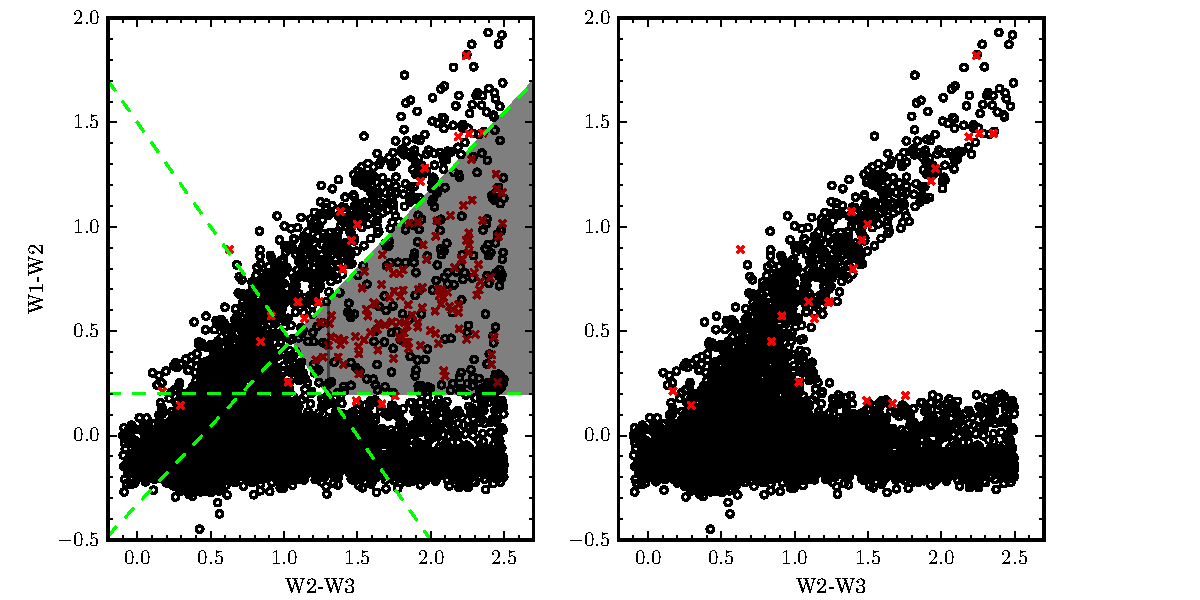
\includegraphics[width=6.5in]{figs/remove_ysos.pdf}
\caption{YSOs (\emph{red x}) and OGLE-III AGBs (\emph{black o}) in the LMC before (\emph{left}) and after (\emph{right}) the application of YSO exclusion criteria in equations \ref{eq:yso_criteria1}-\ref{eq:yso_criteria3}. Dashed green lines outline the bounds for the YSO exclusion criteria, whose area is shaded in black.\label{fig:ysos_lmc}}
\end{figure}

\subsection{Removing RGBs from WISE Color-Color Space}\label{sec:kill_rgbs}
From [cite that Sosynski paper] we see that in the LMC RGB stars overlap with AGBs in color-color and period-luminosity space, and are very difficult to disentangle from AGB stars. However, they are differentiated by the color-corrected magnitudes of TRGB stars and confidence in a narrow-enough distance distribution that these magnitudes can serve a similar purpose as an absolute magnitude--reference magnitudes where the TRGB can be identified and cut. Since we don't have the luxury of known absolute magnitudes or distances for AGB candidates in the Milky Way, we instead use the OGLE-III RGB sample to estimate where they would be in color-color space.

We begin by convolving the color-color criteria of equations~\ref{eq:criteria1} \& \ref{eq:criteria2} with the YSO exclusion critieria in \ref{eq:yso_criteria1}-\ref{eq:yso_criteria3}, yielding 603 LMC RGB stars. 
Even with this grand reduction in the population of RGB stars in our sample, we're still left with 7.97\% contamination after excluding YSO stars. This calls for a specific removal of RGB stars from the sample, so we sought to find where they are most concentrated and easiest removed without adversely affecting sample completeness.

Figure~\ref{fig:rgbs_lmc} shows the distribution of the resulting RGB star sample with respect to the AGB star sample in the LMC in four colors. 
We find that RGB stars overlap with AGB stars in a narrow sequence with the overwhelming majority falling under $J-K_s < 1.35$. In order to reduce the contamination from these objects in our candidate sample, we impose the following cut:

\begin{figure}[h]
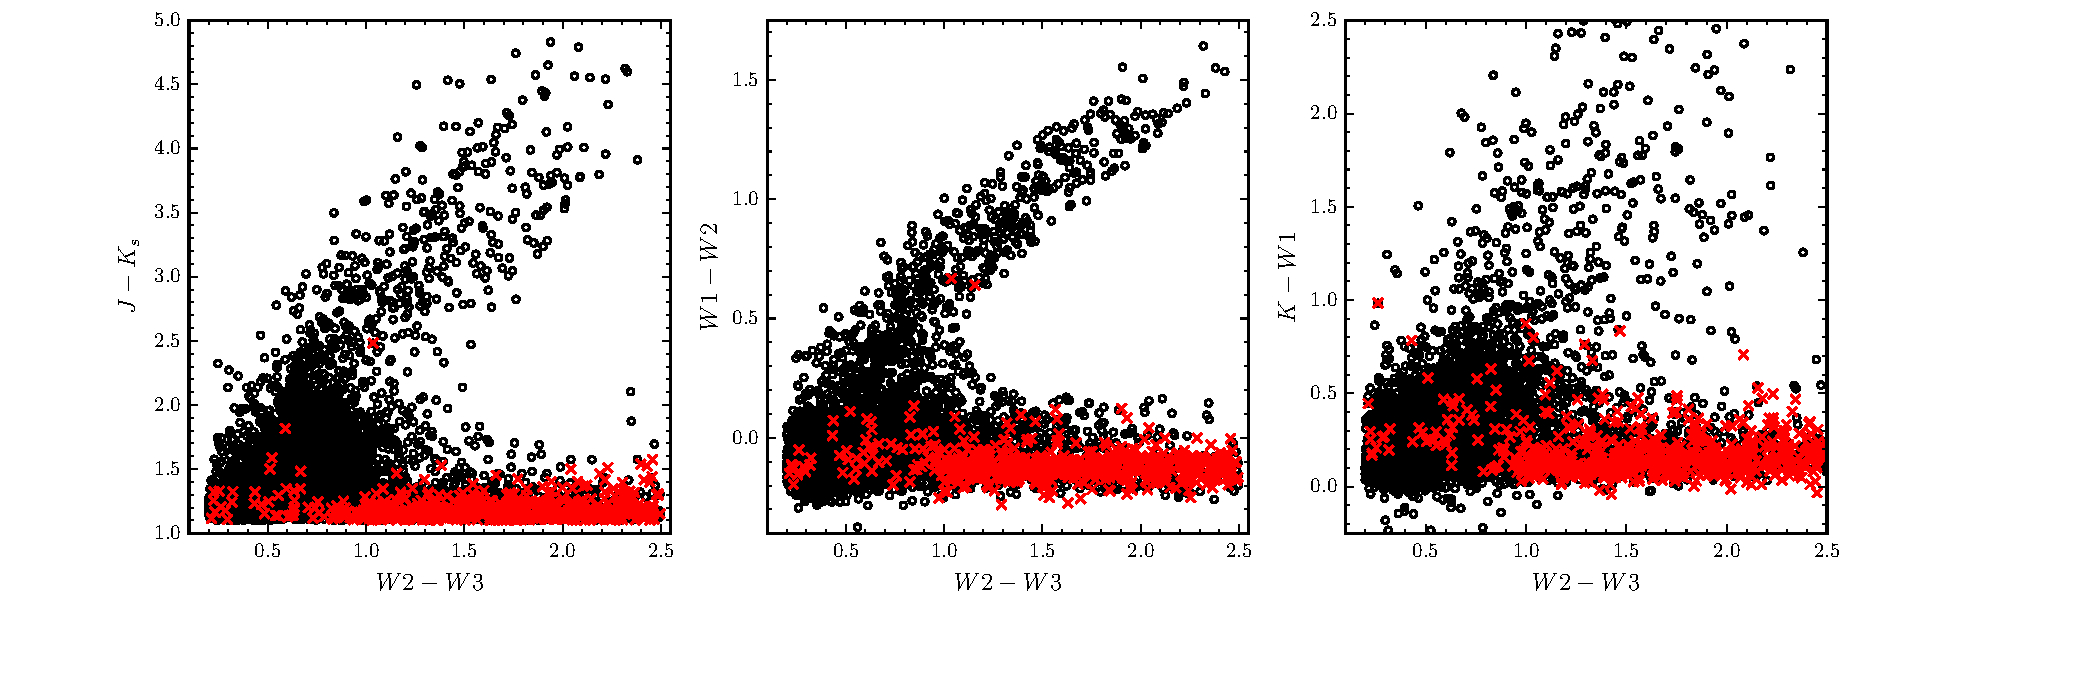
\includegraphics[width=6.5in]{figs/agbs_rgbs_color.pdf}
\caption{OGLE-III RGBs (\emph{red x}) and OGLE-III AGBs (\emph{black dot}) in the LMC. 
\label{fig:rgbs_lmc}}
\end{figure}

\begin{align}
(J-K_s) > 1.35 \text{ for } (W2-W3) > 0.8.\label{eq:rgb_criteria}
\end{align}

\noindent This new criterion results in an LMC AGB star completeness of 71.14\%, while reducing the RGB star contamination down to 1.05\%. The resulting distribution is seen in Figure~\ref{fig:rgbs_after_cut}.


\begin{figure}[h]
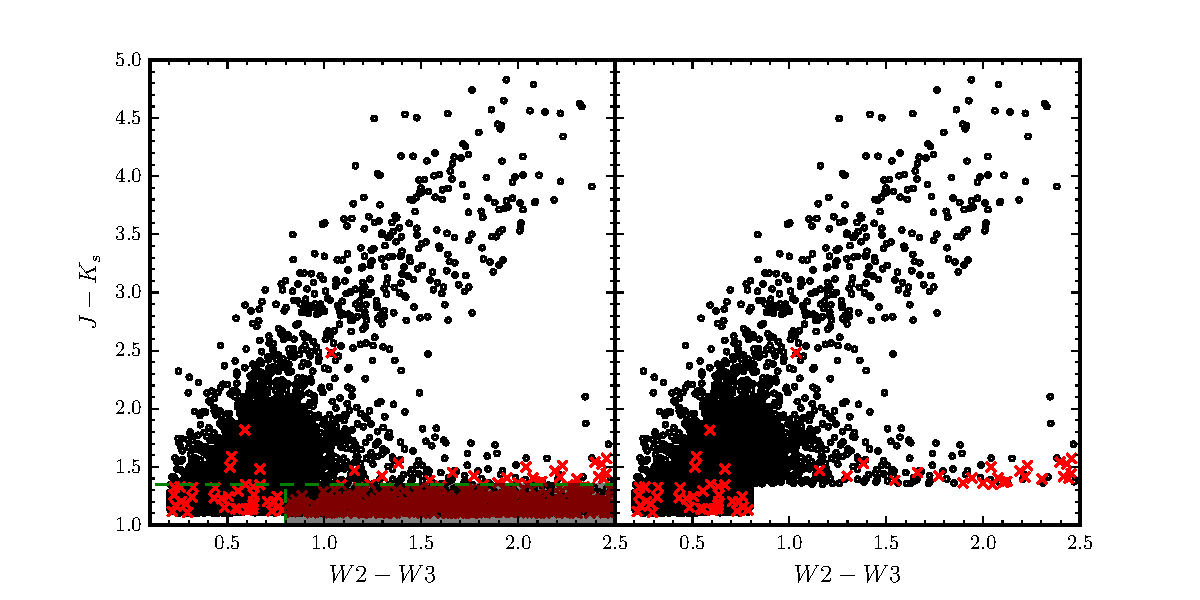
\includegraphics[width=6.5in]{figs/remove_rgbs.pdf}
\caption{OGLE-III RGBs (\emph{red x}) and OGLE-III AGBs (\emph{black dot}) in the LMC before (\emph{left}) and after (\emph{right}) the application of equation~\ref{eq:rgb_criteria}. 
\label{fig:rgbs_after_cut}}
\end{figure}

\subsection{Post-processing Filter}
Using the criteria in equations~\ref{eq:criteria1}-\ref{eq:rgb_criteria}, we selected AGB candidates from the ALLWISE-2MASS database. We recovered 1,383,366 candidates, an almost full order of magnitude over the number estimated by [XXX CITE JACKSON, IVEZIC, AND KNAPP 2002XXX] for the entire Milky Way. Suspecting that we hadn't fully accounted for the contribution to the candidate sample from naked stars, we reconcile this discrepancy by adding one final cut motivated by Figure 4 of [XXX CITE NIKUTTA ET AL 2014 XXX]. In that figure, stars from SDSS with $W1 < 15.8$ are plotted in $W1$ vs $(W1-W2)$, showing a median $(W1-W2)$ of -0.04 dex. With that in mind, we remove objects with $(W1-W2) < -0.04$, retaining a final  population of 306,793 candidate AGB stars.





%In creating color-color criteria to generate a catalog of AGB candidates, we seek to maximize AGB completeness while minimizing contamination from non-AGB objects to beneath the 1\% level.
%
%The color-color criteria for AGB selection are as follows:
%\begin{align} 
%	(J-K_s) > 1.1\label{eq:criteria1}\\
%	(W2-W3) > 0.3\label{eq:criteria2}\\
%	(W3-W4) < -0.83(W2-W3) + 3.37\label{eq:criteria3}
%\end{align}
%The criteria in (\ref{eq:criteria1}) and (\ref{eq:criteria2}) are primarily concerned with rejecting objects from the stellar locus, and other objects whose NIR spectra are dominated by the Rayleigh-Jeans tail. (\ref{eq:criteria3}) also rejects stars from the stellar locus, but primarily functions to remove IR-bright extragalactic sources.
%
%We also experiment with other criteria to focus more closely on the high-reliability AGB population, instead of trying to capture the most AGB-like objects. These criteria are as follows:
%\begin{align} 
%	(W1-W2) < 1\label{eq:criteria4}\\
%	(W2-W3) < 1\label{eq:criteria5}
%\end{align}
%Criteria (\ref{eq:critera4}) restricts NIR excesses. Criteria (\ref{eq:criteria5}) primarily removes extragalactic sources, while only slightly cutting into the distribution of known AGB stars.
%
%\noindent Sample completeness $\eta$ is defined as
%\begin{eqnarray*}
%\eta &=& \frac{N - n_\text{missed}}{N}
%\end{eqnarray*}
%where $N$ is the total number of objects in the sample, and $n_\text{missed}$ is the number of objects outside of the applied boundaries. Figure~\ref{fig:completeness} shows the distribution of sample completeness amongst AGB sources after the application of the above criteria. The vast majority (79.07\%) of Galactic AGB stars is recovered after criteria (\ref{eq:criteria1}), (\ref{eq:criteria2}), and (\ref{eq:criteria3}) are applied. The largest losses occur at the edges of the Galactic disk ($\lvert b\rvert\approx10^\circ$) and in regions of high stellar number density both in the Galaxy and the Magellanic Clouds. In the color-color diagrams, selection completeness degrades near the borders of the selection area, as objects that straddle these boundaries may exhibit enough emission in other color-color spaces to be removed by our criteria. Of the remaining sample of 5,709 objects, 52.94\% lie within the disk ($\lvert b\rvert<10^\circ$).
%
%\begin{table}[h]
%    \begin{center}
%        \caption{Samples Recovered wih Application of Criteria (\%)}
%        \scalebox{0.85}{
%            \begin{tabular}{l r r r r r r r r r r r r}
%\hline
%Object Type & Reduced & (1) & (2) & (3) & (1,2) & (1,2,3) & | & \textbf{(4)} & \textbf{(5)} & \textbf{(1,2,4)} & \textbf{(1,2,5)} & \textbf{(1,2,4,5)}\\
%\hline
%All AGBs & 7220 & 95.15 & 84.89 & 95.21 & 82.62 & 79.07 & | & \textbf{94.22} & \textbf{88.82} & \textbf{77.05} & \textbf{72.71} & \textbf{71.14}\\ 
%O-rich AGB & 3147 & 98.98 & 100.00 & 100.00 & 98.98 & 98.98 & | & \textbf{98.44} & \textbf{97.33} & \textbf{97.43} & \textbf{96.31} & \textbf{94.88}\\ 
%C-rich AGB & 540 & 99.26 & 99.81 & 99.26 & 99.07 & 98.33 & | & \textbf{57.59} & \textbf{63.33} & \textbf{56.85} & \textbf{62.59} & \textbf{54.44}\\ 
%Unclassed AGB & 3533 & 91.11 & 69.15 & 90.32 & 65.53 & 58.39 & | & \textbf{96.07} & \textbf{85.14} & \textbf{61.99} & \textbf{53.24} & \textbf{52.53}\\ 
%DR12 SSPP & 67508 & 76.16 & 99.16 & 0.91 & 76.07 & 0.05 & | & \textbf{86.05} & \textbf{0.89} & \textbf{65.67} & \textbf{0.03} & \textbf{0.03}\\ 
%DR7 LRG & 84 & 96.43 & 100.00 & 0.00 & 96.43 & 0.00 & | & \textbf{89.29} & \textbf{0.00} & \textbf{85.71} & \textbf{0.00} & \textbf{0.00}\\ 
%QSO & 3783 & 73.54 & 99.97 & 0.13 & 73.54 & 0.11 & | & \textbf{34.50} & \textbf{0.11} & \textbf{27.54} & \textbf{0.08} & \textbf{0.08}\\ 
%Galaxy & 42066 & 78.55 & 100.00 & 0.01 & 78.54 & 0.00 & | & \textbf{96.39} & \textbf{0.01} & \textbf{75.31} & \textbf{0.00} & \textbf{0.00}\\ 
%AGN & 1011 & 79.33 & 100.00 & 0.00 & 79.33 & 0.00 & | & \textbf{96.34} & \textbf{0.00} & \textbf{75.87} & \textbf{0.00} & \textbf{0.00}\\ 
%
%\hline
%                \label{tab:criteria}
%            \end{tabular}}    
%    \end{center}
%\end{table}
%
%
%\begin{figure}[h]
%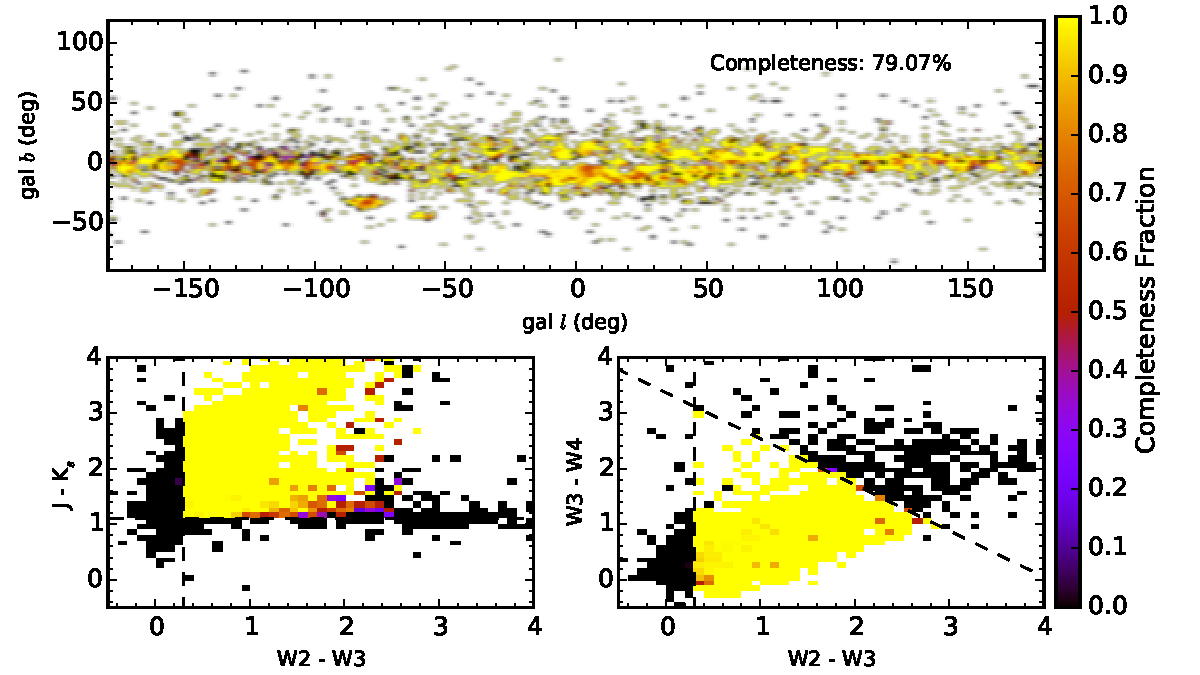
\includegraphics[width=6.7in]{figs/completeness_map.pdf}
%\caption{Sample selection completeness maps in ($l,b$) space (\emph{top}) and the color-color space of our selection criteria (\emph{bottom}). Color scale shows the completeness fraction per bin, with 4-deg$^2$ bins on the Galactic map and 0.1 dex bins on each axis of the color-color diagrams. Selection criteria are shown as dashed lines.\label{fig:completeness}}
%\end{figure}
%
%\cite{2013sdmm.book.....I} defines sample contamination as
%\begin{eqnarray*}
%\epsilon &=& \frac{n_\text{spurious}}{n_\text{selected}}.
%\end{eqnarray*}
%where $n_\text{spurious}$ is the number of spurious sources and $n_\text{selected} = N + n_\text{spurious}$. The contamination map is shown in Figure~\ref{fig:contamination}. Most bins in Figure~\ref{fig:contamination} exhibit 0\% contamination, with the overall contamination level at 0.38\%. What contaminants do remain exist primarily at the very fringes of the AGB star distribution in ($J-K_S$) vs ($W2 - W3$) space and near the redder boundary in ($W3-W4$) vs ($W2 - W3$), where bluer extragalactic sources creep into the selection region. The results of the applied criteria on both the collective AGB and contaminant samples are summarized in Table~\ref{tab:completeness}. 
%
%We note that while we do achieve a low rate of contamination, most of our contaminant sources are out of the plane of the Galaxy, while many of our \agb\, sources are within the Galactic disk. Considering how our extragalactic contaminant sources are from various iterations of \sdss, we know that their spatial distributions should be effectively uniform across the sky {\color{red} [cite me]}. For contaminants unaffected by interstellar reddening, they would occupy the same regions of color-color space already marked by our existing contaminant sample, and would similarly be removed by (\ref{eq:criteria1}), (\ref{eq:criteria2}), and (\ref{eq:criteria3}). This would produce the same zero-level contamination for all extragalactic sources aside from QSOs. We can adopt a QSO spatial density by dividing the total number of spectroscopically identified QSOs by the covered area on the sky. Using this, we recover a QSO spatial density of {\color{red} some number per square degree}. Using that density, and assuming ubiquity of sources on the sky, complete detection of QSOs {\color{red} down to some magnitude limit}, and a lack of interstellar reddening, we can estimate a maximum QSO contamination fraction of {\color{red} some number}. We use this number to report our QSO contamination fraction in Table~\ref{tab:completeness}, as QSOs significantly affected by interstellar reddening would exist further outside of the limits of (\ref{eq:criteria1}), (\ref{eq:criteria2}), and (\ref{eq:criteria3}). A more rigorous study of QSO spatial density is outside the scope of this paper.
%
%The remaining contaminant sample is from the \sdss\, DR12 SSPP, with the number of remaining species found within shown in Figure~\ref{fig:sspp_histo}. {\color{red} the figures don't match up with each other. The number of red stars on the right side of the fig are significantly less than those in the histogram. Reconcile this.}
%
%\begin{figure}[h]
%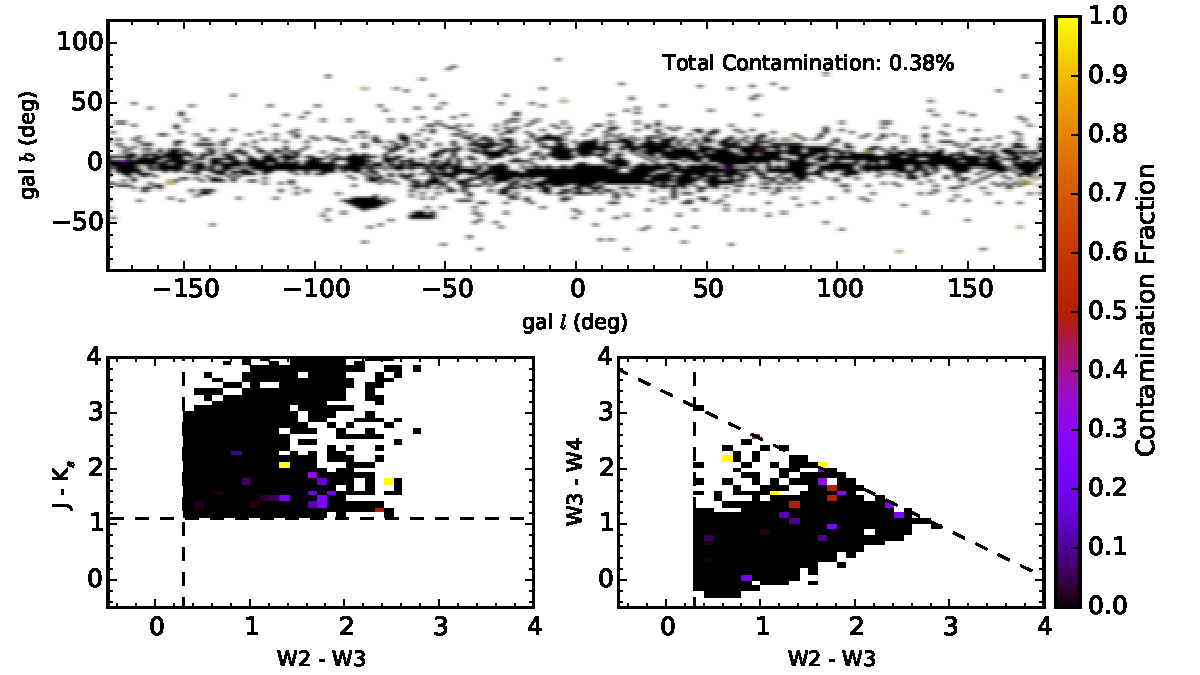
\includegraphics[width=6.7in]{figs/contamination_map.pdf}
%\caption{Sample contamination in Galactic ($l,b$) space (\emph{top}) and color-color space (\emph{bottom}). Boundaries and binning the same as Fig~\ref{fig:completeness}.\label{fig:contamination}}
%\end{figure}
%
%\begin{figure}[h]
%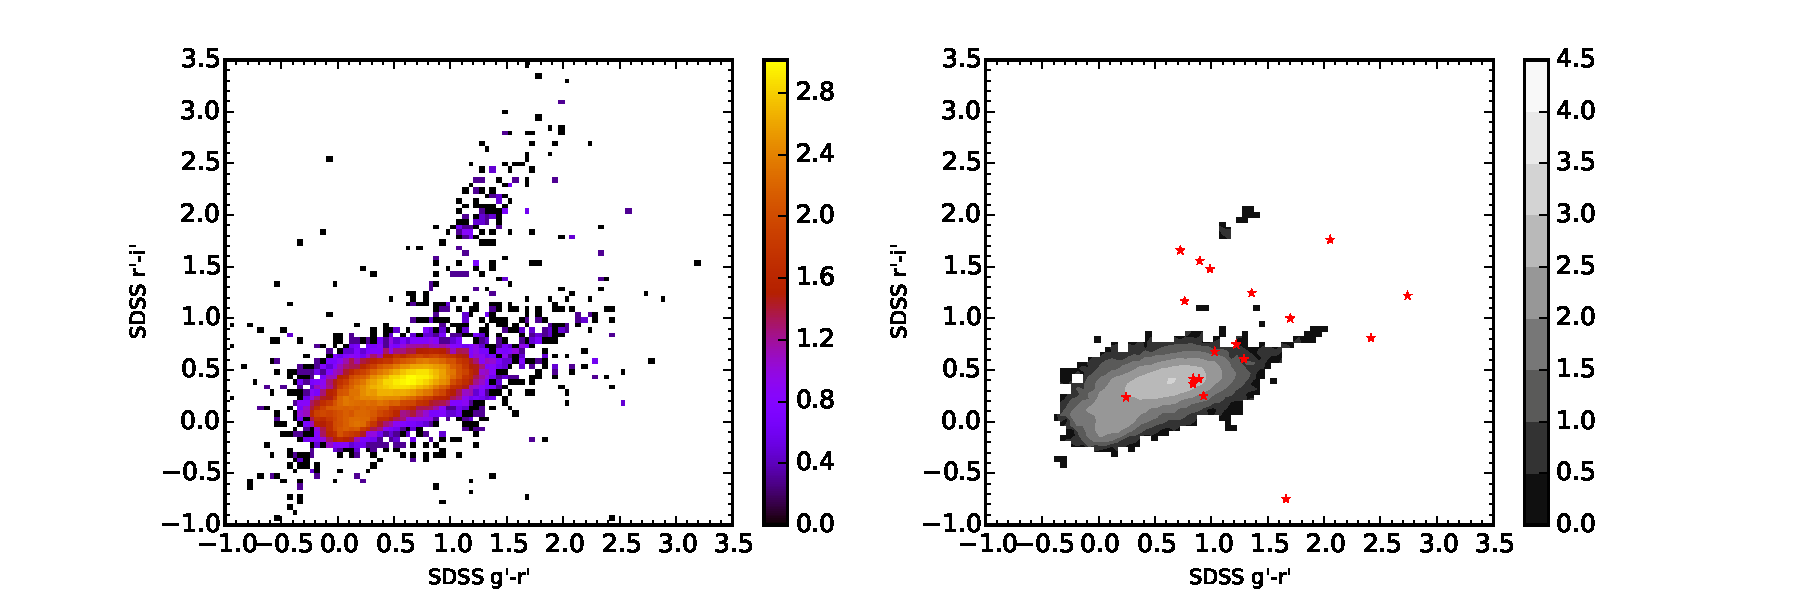
\includegraphics[width=6.7in]{figs/contaminating_sspp_objects.pdf}
%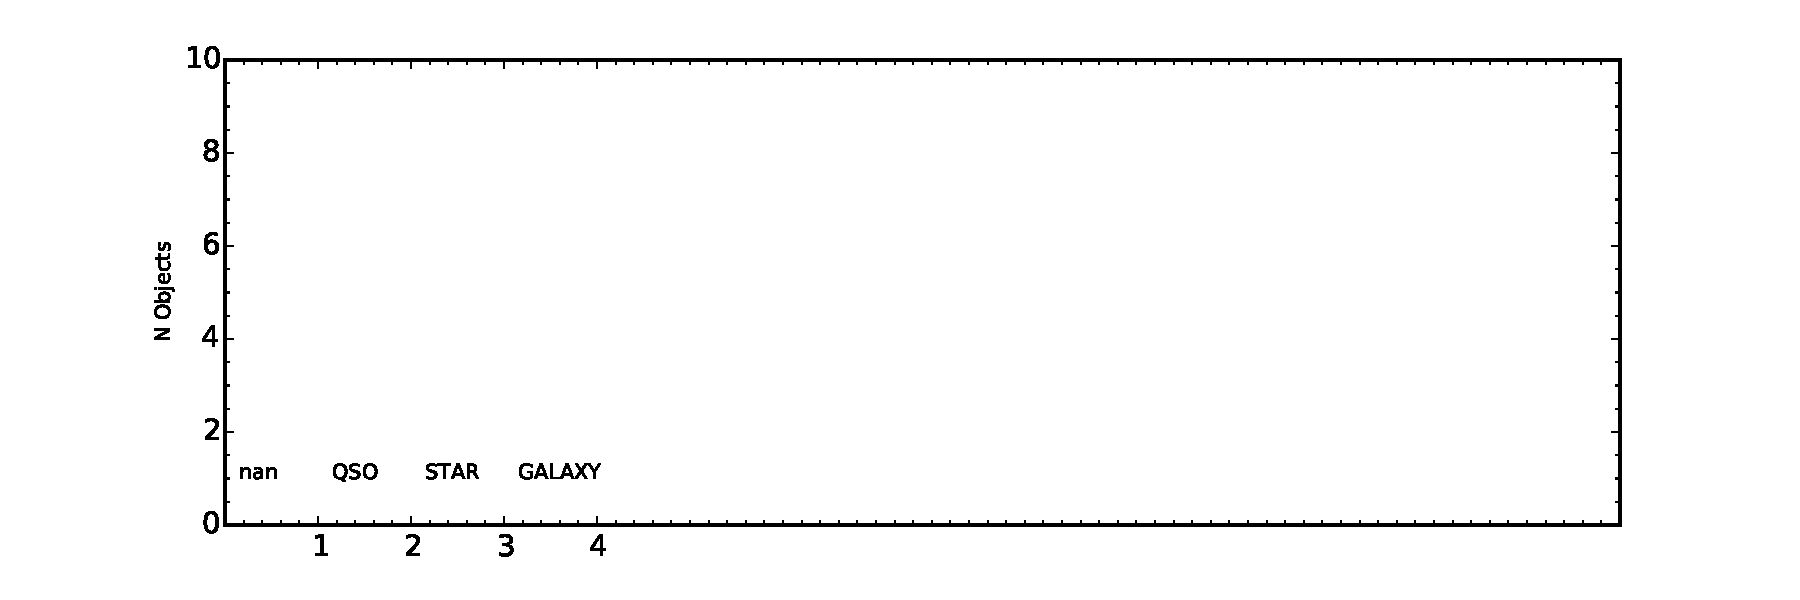
\includegraphics[width=6.7in]{figs/contaminating_sspp_objects_classes.pdf}
%\caption{Some histogram\label{fig:sspp_histo}}
%\end{figure}
%
%%One large issue with the boundaries are the O-rich AGB stars.  Either the objects from the OGLE O-rich AGB star catalog were mostly mis-matched to WISE, taking on colors of the stellar locus, or the issue is more physical.  It could be that the warm O-rich AGB photospheres are still visible and not heavily enshrouded in dust, thus appearing similar to Main Sequence stars in the NIR. Previous work on warm O-rich AGB stars has shown that their circumstellar shells are not prominent, and their NIR photometry reflects the Rayleigh Jeans tail of a cool 2000-4000K blackbody \citep{1974ApJ...189...89D}. 
%
%\begin{table}[h]
%    \begin{center}
%        \caption{Sample Selection Completeness and Contamination}
%        \scalebox{0.85}{
%            \begin{tabular}{l c c c c c c}
%		\hline
%		Population & SIMBAD AGB* & C* & Mira & OH/IR & S* \\ 
%		Completeness & 89.62\% & 72.11\% & 95.62\% & 39.53\% & 22.31\% \\ 
%		\hline
%		Population & MACHO seq1 & seq2 & seq3 & seq4 \\ 
%		Completeness & 88.45\% & 81.08\% & 28.77\% & 14.75\% \\ 
%		\hline
%		Population & OGLE-III C-rich & O-rich & \textbf{All AGB Stars} \\ 
%		Completeness & 73.09\% & 70.68\% & \textbf{79.07\%} \\ 
%		\hline
%		Population & DR12 SSPP & DR7 LRG & Galaxies & QSO & AGN \\ 
%		Contamination & 0.56\% & 0.00\% & 0.00\% & 0.07\% & 	0.00\% \\ 
%		\hline
%
%                \label{tab:completeness}
%            \end{tabular}}    
%    \end{center}
%\end{table}
%

